\section{Endmontage Radio und Taschenlampe}

\subsection{Bestücken und Löten der Taschenlampe}
Die Taschenlampe wurde speziell so konstruiert, dass auch die SMD-Bauteile problemlos von Hand gelötet werden können.
Dabei spielt vor allem die Größe der Lötpads eine entscheidende Rolle.
Während beim Reflowlöten möglichst kleine Pads verwendet werden, sind diese beim Handlöten etwas größer, um genügend Spielraum für den Lötkolben zu gewährleisten.\\
\\
Zuerst werden die SMD-Bauteile auf die Unterseite der Platine gelötet.
Diese Reihenfolge erleichtert die Arbeit, da die Platine flach auf der Arbeitsfläche liegt, was die genaue Positionierung der kleinen Bauteile unterstützt.
Danach erfolgt das Verlöten der Duschkontaktierungen.
Diese Arbeitsschritte sind in der Regel einfacher, da die größeren Bauteile stabiler sind und während des Lötprozesses nicht verrutschen können.\\
\\
Nach dem Verlöten der verdrahteten Bauteile werden überstehende Drähte, z.B. von Leuchtdioden und Spulen, mit einem Seitenschneider entfernt.\\
\\
Beim Zusammenbau der Taschenlampe ist es wichtig, die Reihenfolge der Arbeitsschritte einzuhalten. Zuerst werden die SMD-Bauteile verlötet, dann die bedrahteten Bauteile.
Die Polarität der Schottky-Diode und der Leuchtdioden ist zu beachten.
Außerdem dürfen Kondensatoren nicht zu lange der Hitze ausgesetzt werden, um Schäden zu vermeiden. Nach dem Löten wird die Taschenlampe auf Funktion geprüft.

\begin{figure}[H]
    \centering
    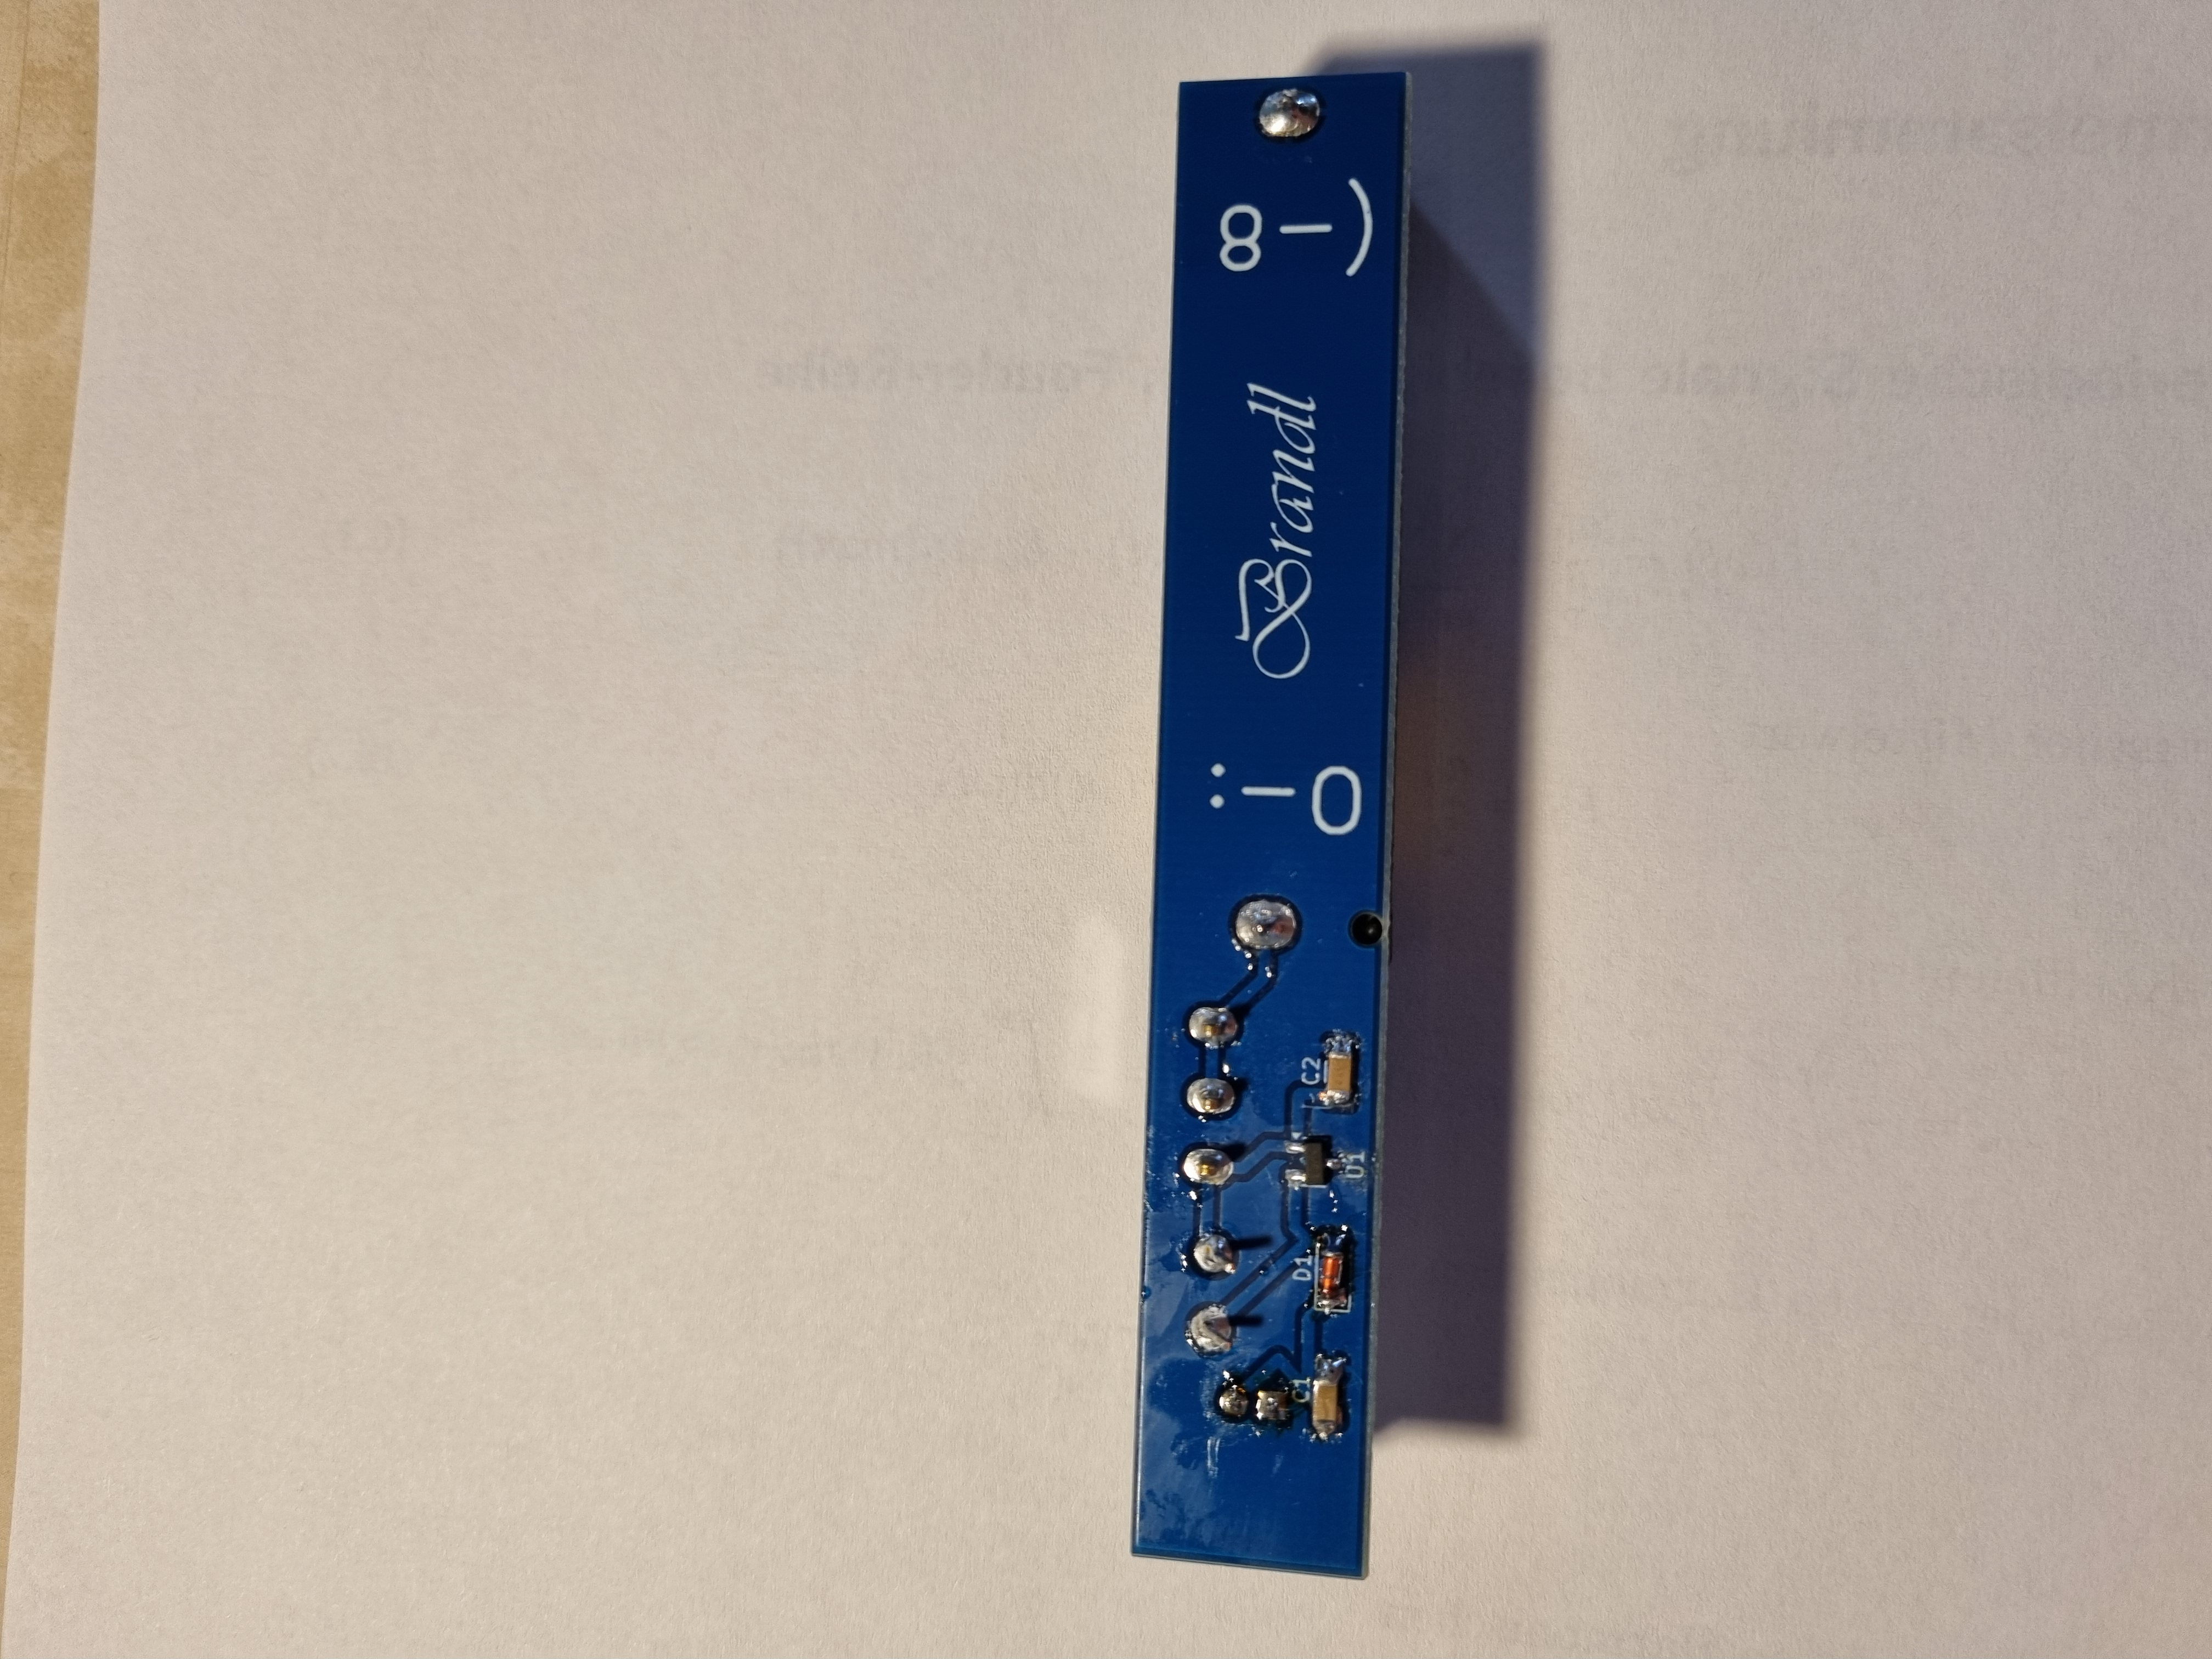
\includegraphics[width=0.8\textwidth]{\figdir/Unterseite der Taschenlampe}
    \caption{Unterseite der Taschenlampe}
    \label{fig: Abbildung 11}
\end{figure}

\begin{figure}[H]
    \centering
    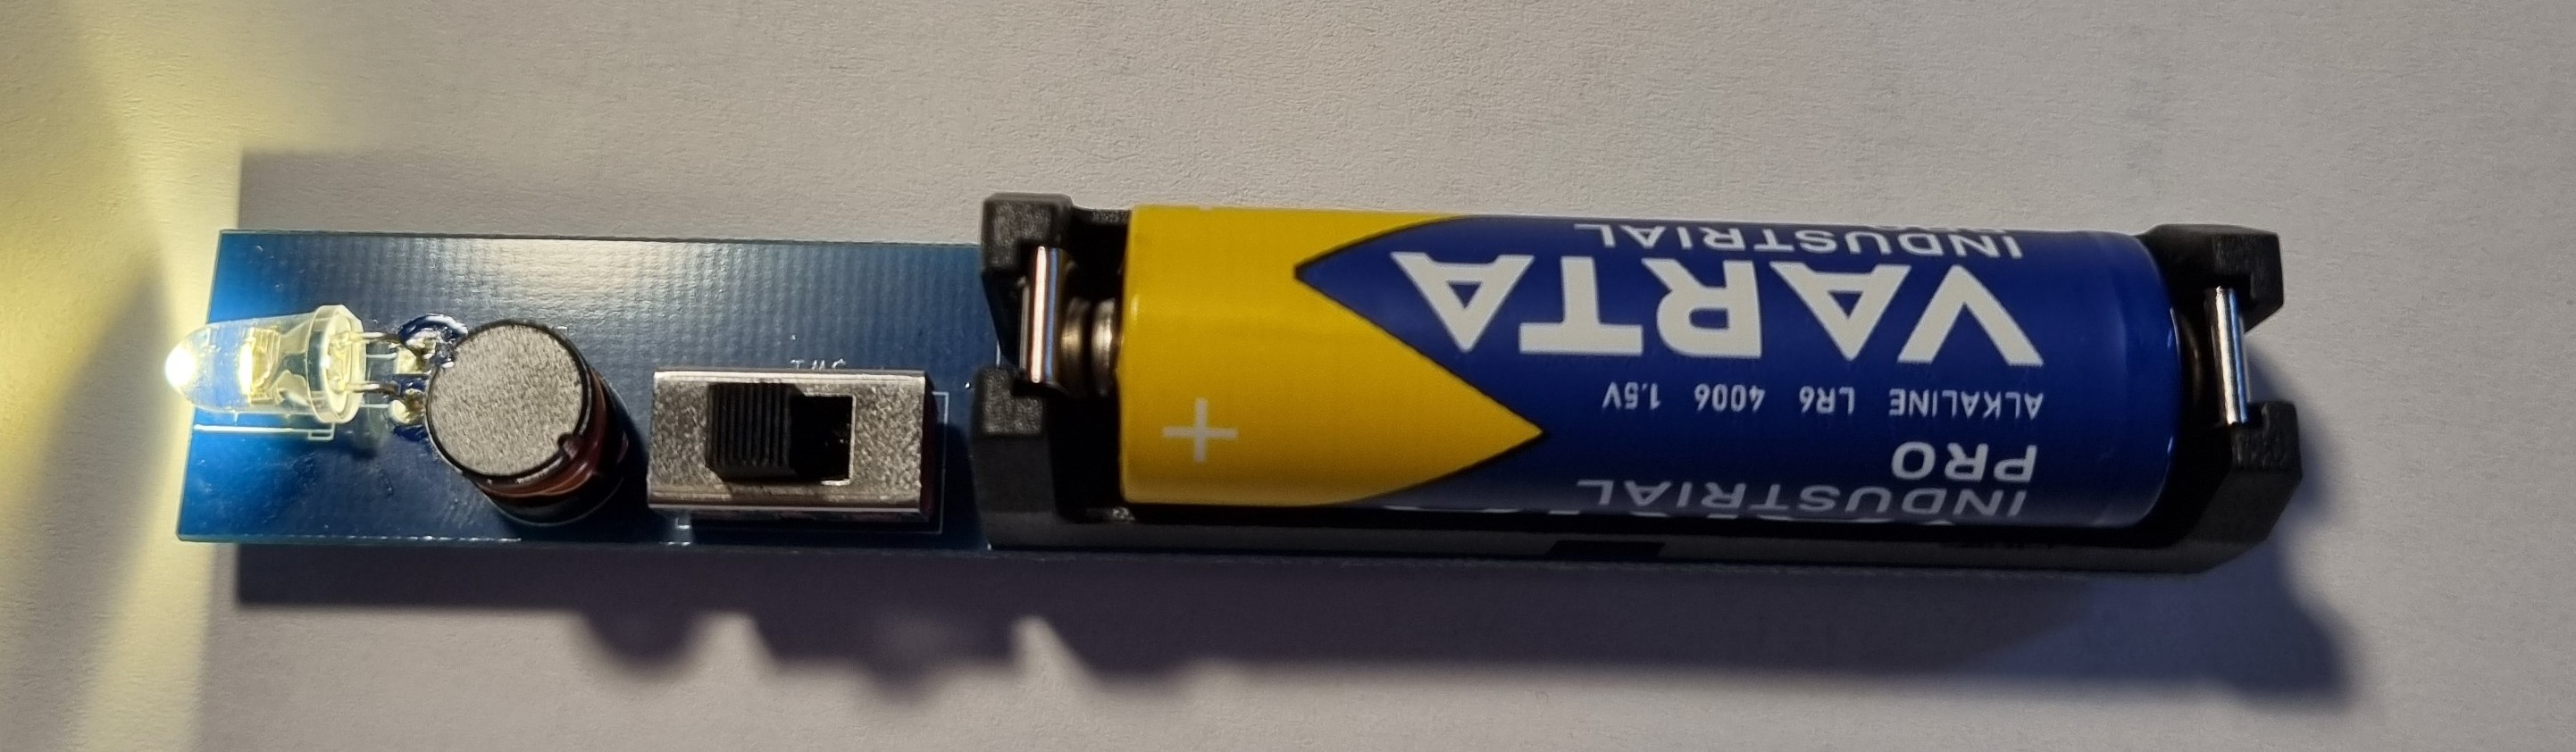
\includegraphics[width=0.8\textwidth]{\figdir/Oberseite der Taschenlampe}
    \caption{Oberseite der Taschenlampe}
    \label{fig:fig: Abbildung 12}
\end{figure}

\subsection{Bestücken und Löten des Radios}
Die Bestückung der Leiterplatte erfolgt in einer Kombination aus manuellen und maschinellen Verfahren.
Auch für das Auftragen der Lötpaste werden verschiedene Methoden verwendet.\\
\\
Auf der Vorderseite der Radioplatine befinden sich sechs Leuchtdioden und zwei Lautsprecher.
Aufgrund der vergleichsweise geringen Anzahl von Bauteilen wird hier die Lotpaste mit einem Handdispenser aufgetragen, der über Druckluft gesteuert wird.
Ein Fußpedal regelt den Luftdruck und sorgt dafür, dass genau die richtige Menge Lotpaste auf die Pads aufgetragen wird.
Bei den Lautsprecherpads wird die Paste in Schleifen aufgetragen, bei den LED-Pads genügen einzelne Striche.

\begin{figure}[H]
    \centering
    \includegraphics[width=0.8\textwidth]{\figdir/Handdispenser beim Auftragen der Lötpaste}
    \caption{Handdispenser beim Auftragen der Lötpaste}
    \label{fig:fig: Abbildung 13}
\end{figure}

\noindent
Nach dem Auftragen der Lotpaste erfolgt die Bestückung der Bauteile mit einem Handbestücker.
Der Greifer erkennt über den Anpressdruck, ob ein Bauteil aufgenommen oder abgelegt wird.
Zusätzlich ermöglicht das Handhabungsgerät das Drehen der Bauteile, während ein Rotationsmagazin die kontinuierliche Zuführung von Bauteilen unterstützt.

\begin{figure}[H]
    \centering
    \includegraphics[width=0.8\textwidth, height = 6cm]{\figdir/Handhabungsgerät}
    \caption{Handhabungsgerät}
    \label{fig:fig: Abbildung 14}
\end{figure}

\newpage
\noindent
Anschließend wird die Vorderseite der Leiterplatte in einem Reflow-Ofen gelötet.
Die Vorheizphase dauert 45 Sekunden, gefolgt von einer Lötphase von 15 Sekunden. Nach dem Löten muss die Leiterplatte zunächst abkühlen, da sie sehr heiß ist.
Damit die bereits gelöteten Bauteile beim zweiten Lötvorgang nicht verrutschen, werden sie zusätzlich mit Klebstoff fixiert.\\
\\
Auf der Rückseite der Leiterplatte wird die Lötpaste mit einer Schablone und einem Rakel aufgetragen.
Dabei muss die Leiterplatte genau unter der Schablone positioniert werden, damit die Paste genau auf den Pads landet.
Andernfalls kann es zu Kurzschlüssen auf den Pads kommen und das Bauteil muss von Hand wieder entfernt und neu verlötet werden.

\begin{figure}[H]
    \centering
    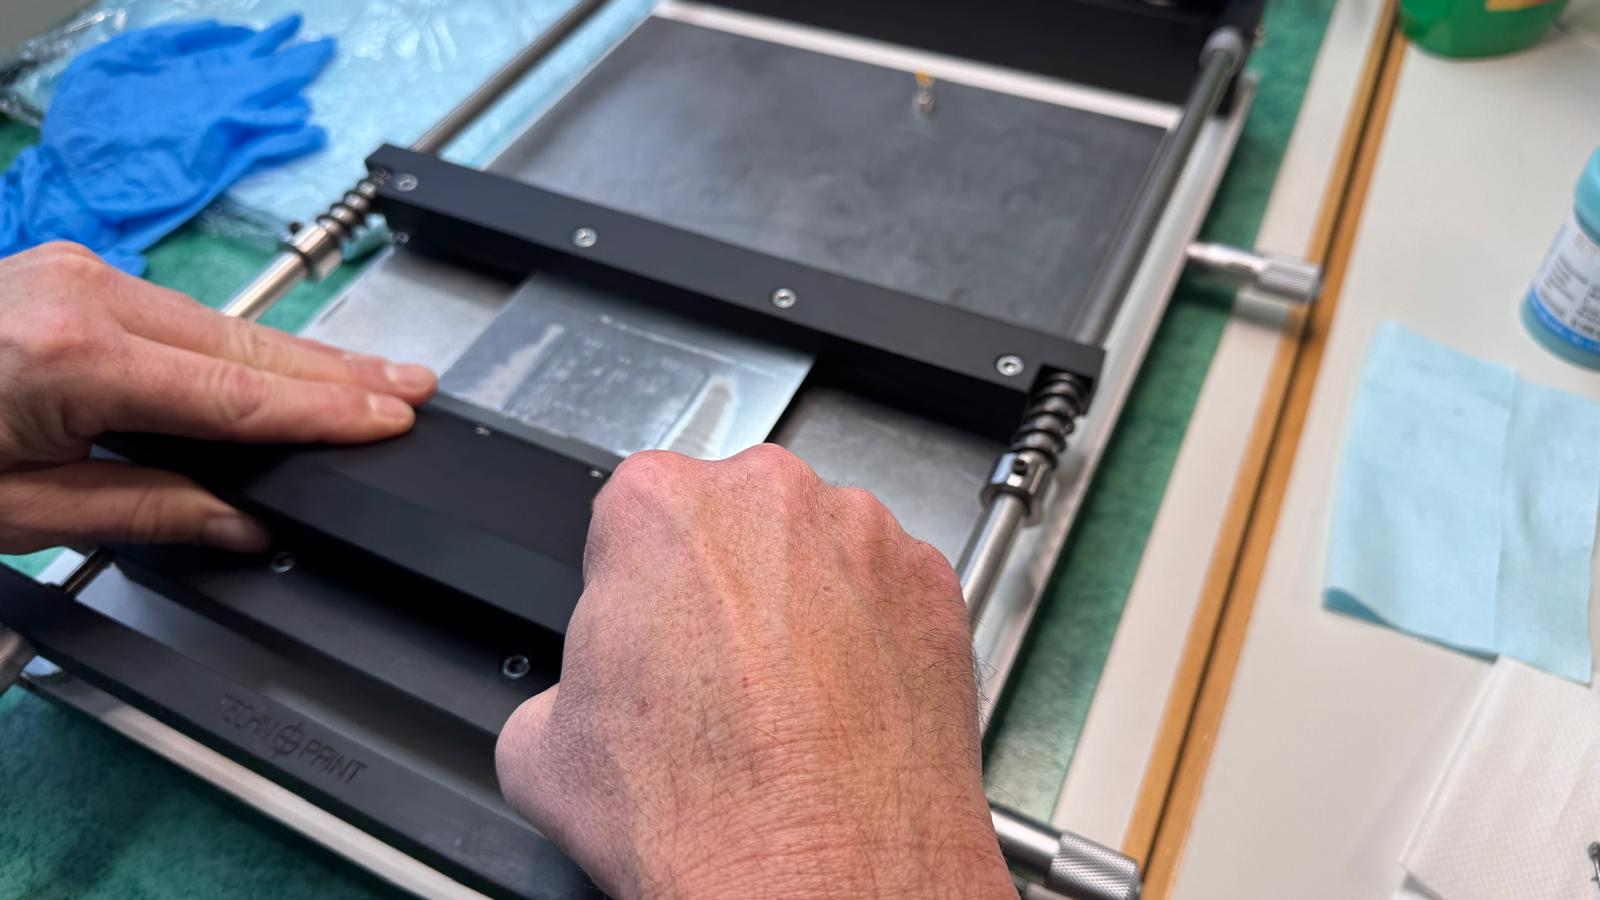
\includegraphics[width=0.8\textwidth]{\figdir/Schablone und Rakel}
    \caption{Schablone und Rakel beim Auftragen der Lötpaste}
    \label{fig:fig: Abbildung 15}
\end{figure}

\newpage
\noindent
Nach dem Auftragen der Paste wird die Leiterplatte in einen Bestückungsautomaten eingelegt.
Dieser erkennt die Positionsmarken und richtet die Leiterplatte entsprechend aus. Die meisten Bauelemente werden automatisch bestückt. Andere Bauteile wie Elektrolytkondensatoren, SMD-Widerstände, Kondensatoren und ICs müssen manuell mit dem Handlinggerät bestückt werden.\\
\\
Die beiden ICs und die Micro-USB-Schnittstelle werden mit Hilfe eines speziellen Kamerasystems platziert.
Dieses macht mit Hilfe von Spiegeln die Kontakte unter den Chips sichtbar und ermöglicht so eine präzise Platzierung.\\
\\
Nach der kompletten Bestückung wird die Radioplatine ein zweites Mal im Reflow-Ofen gelötet.
Anschließend wird die Software zur Programmierung des Funkchips aufgespielt.
Am Anschluss X201 wird die Antenne angeschlossen und die Funtionalität des Radios wird überprüft.

\begin{figure}[H]
    \centering
    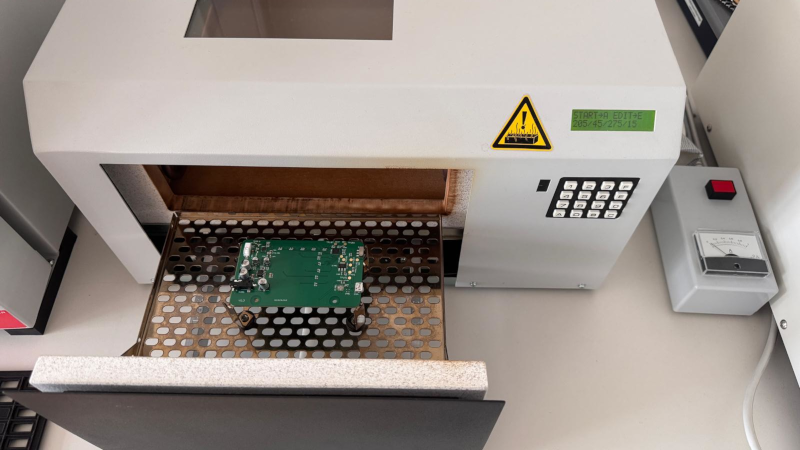
\includegraphics[ width=0.8\textwidth]{\figdir/Radioplatine im Reflowofen}
    \caption{Radioplatine im Reflowofen}
    \label{fig:fig: Abbildung 16}
\end{figure}

\begin{figure}[H]
    \centering
    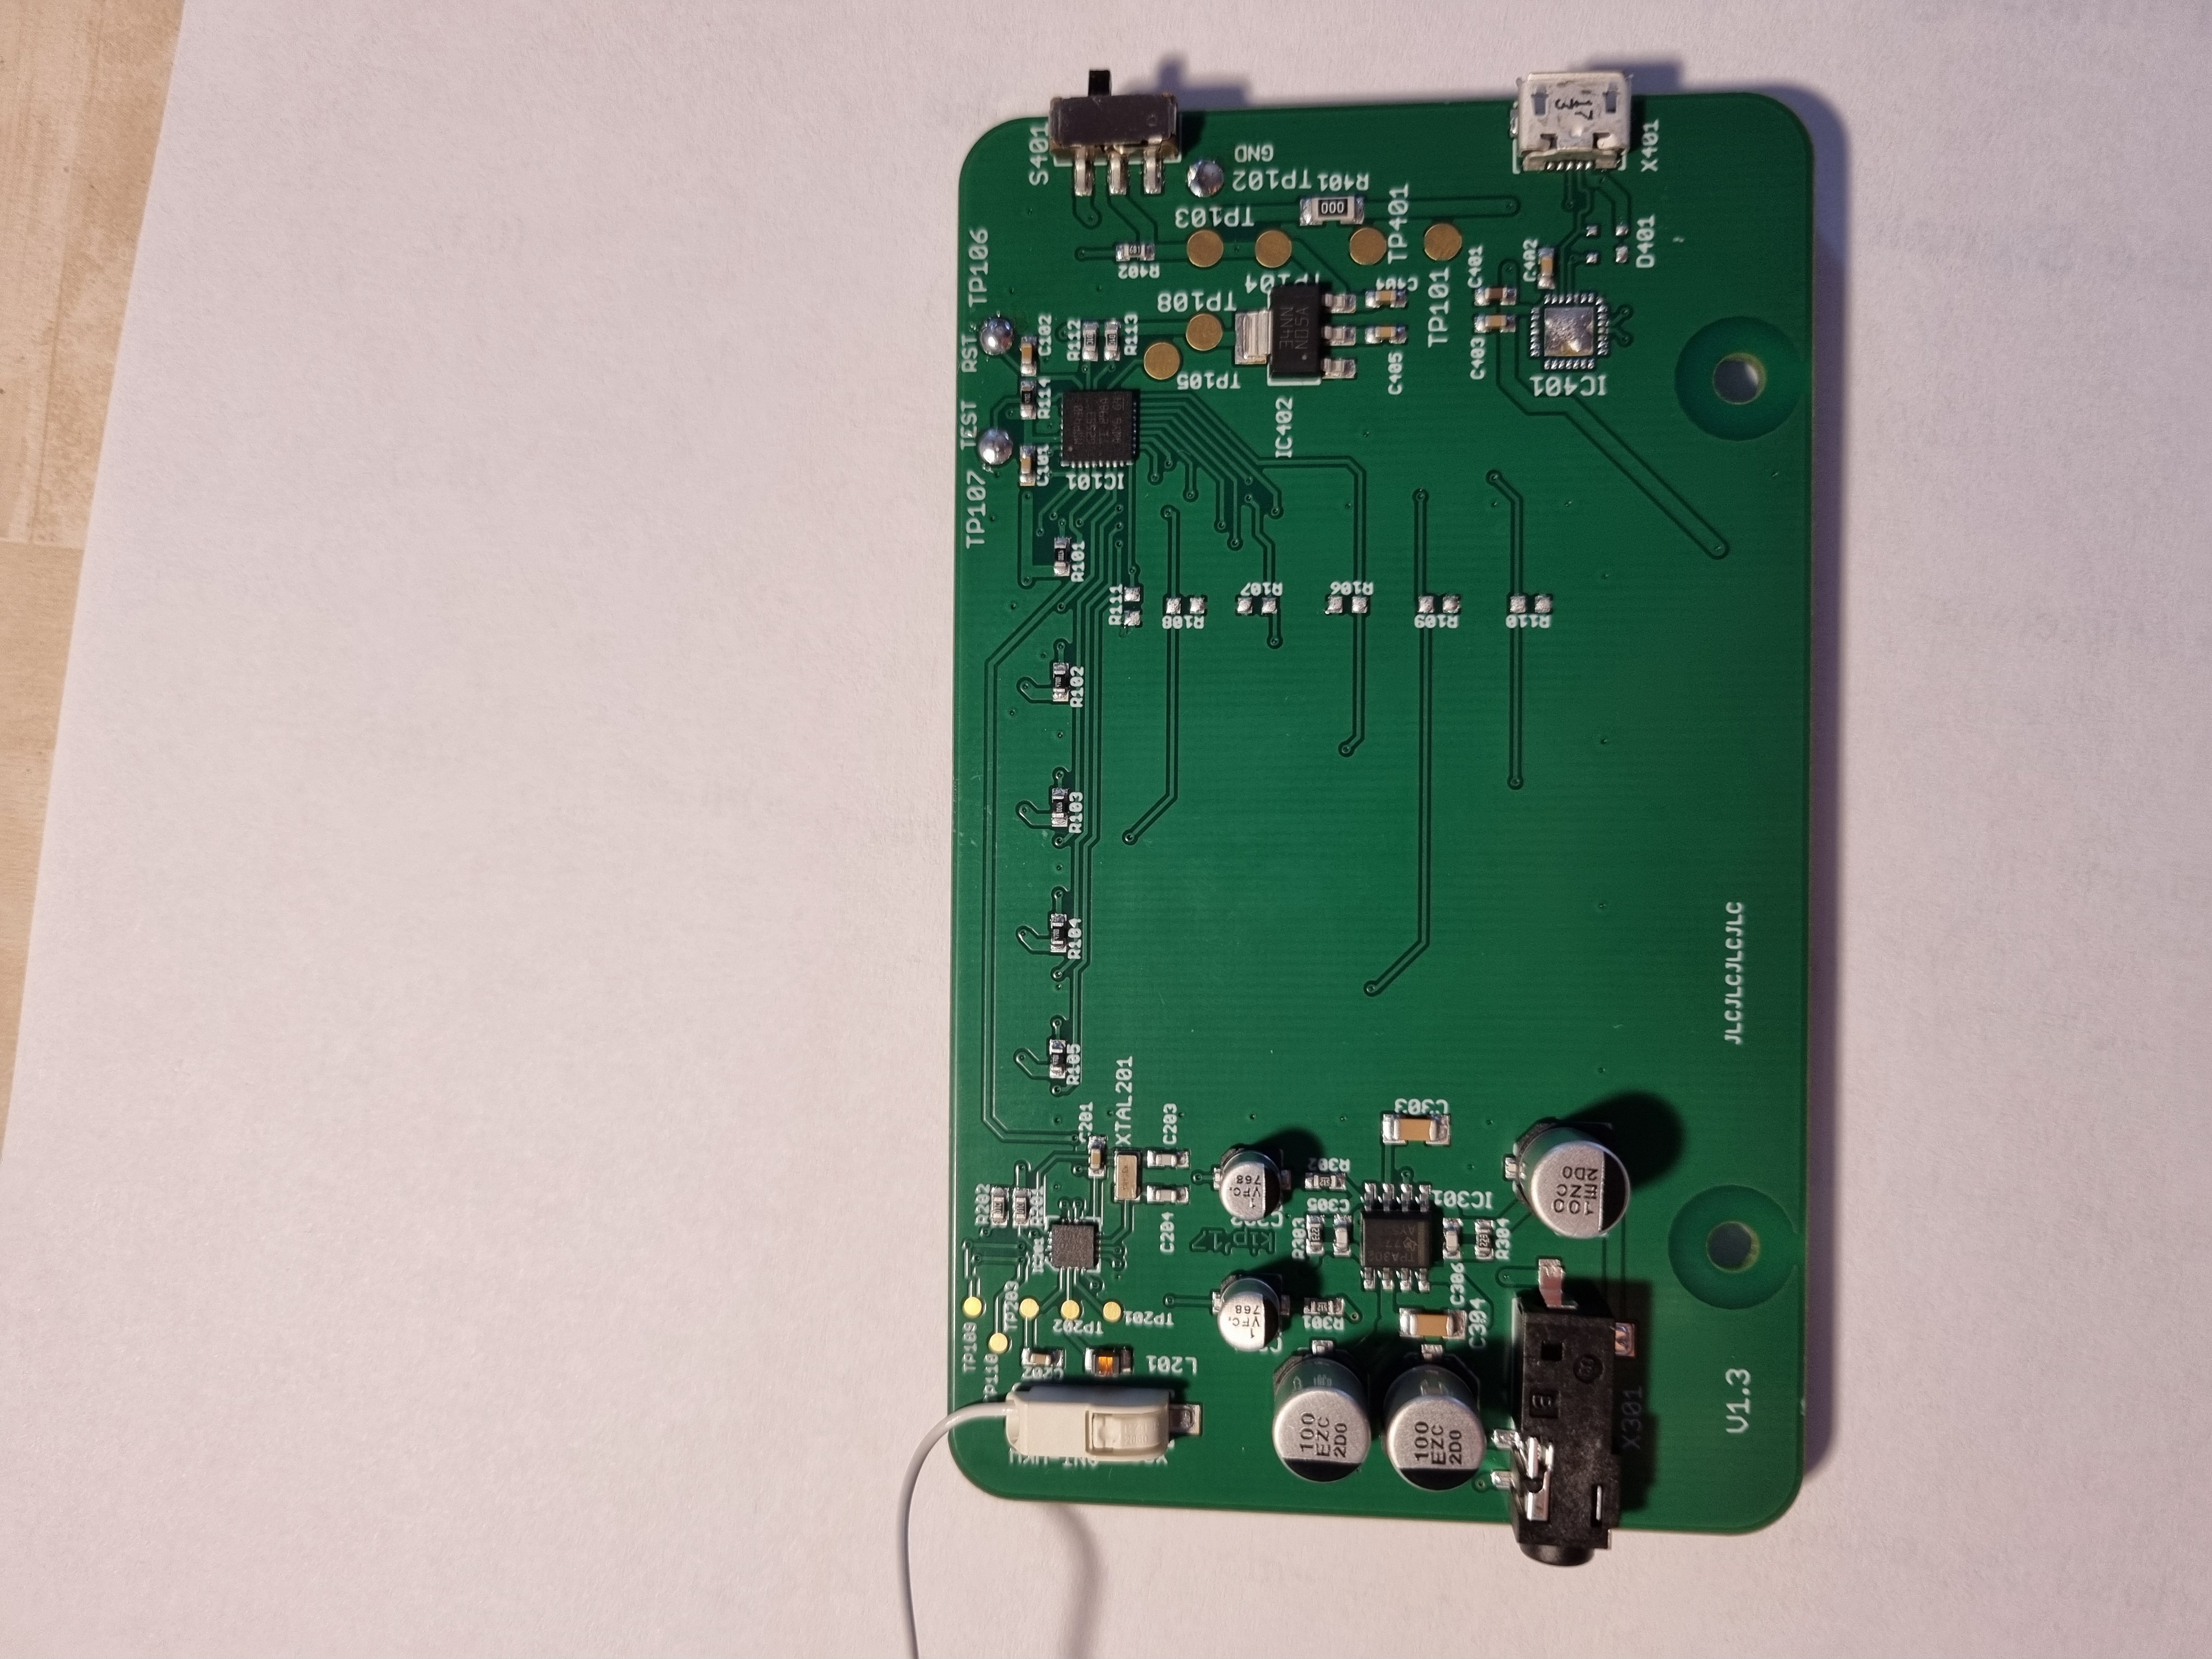
\includegraphics[width=0.8\textwidth, height = 7cm]{\figdir/Radioplatine Unterseite mit angeklemmter Antenne}
    \caption{Radioplatine Unterseite mit angeklemmter Antenne}
    \label{fig:fig: Abbildung 17}
\end{figure}


